\begin{figure}[t]
\centering
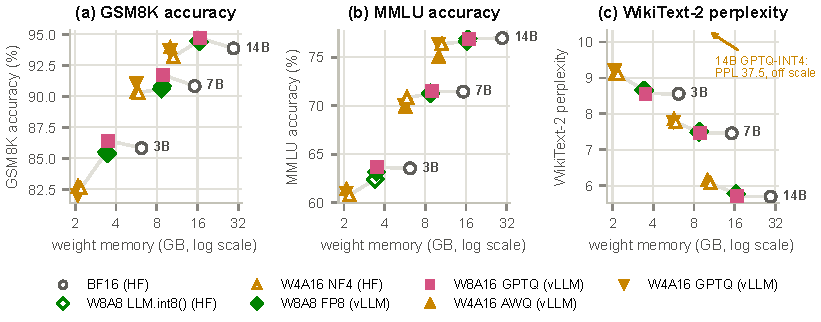
\includegraphics[width=\linewidth]{q4_quality_vs_memory}
\caption{\textbf{Q4: quality against weight memory} for every Qwen2.5 configuration. Lines connect the
configurations of one model size; colours and markers follow the quantization type
(\cref{tab:configs}). A larger model in 4 bits sits above a smaller model in 16 bits, at less memory.}
\label{fig:quality}
\end{figure}

\answer{8-bit formats keep quality. 4-bit formats cost a little, most on small models. The saved
memory is therefore best spent on a larger model.}

\textbf{Noise floor.} The memory and speed gains are worth only as much as the quality they keep. To
judge a change, we first need the noise floor. BF16 on the two stacks disagrees on
\BackendFlipsSeven{} of the 7B model's GSM8K answers, because different kernels round differently, yet
the accuracies differ by only \BackendNoiseSeven{} points (MMLU: \MBackendNoiseSeven).

\textbf{8 bits keep quality.} Measured against this floor, 8-bit formats show no loss. GPTQ-INT8 and
FP8 stay within \EightKernMax{} points of BF16 on both benchmarks for all three sizes; on GSM8K,
\EightSentence{} (\cref{tab:quality_main}). The only measurable 8-bit cost is LLM.int8() on the 3B
model (\IntMMLUThree{} MMLU points, \IntMMLUpThree).

\textbf{4 bits cost a little.} Removing four more bits does cost quality. The 4-bit formats change
MMLU accuracy by \MDFourMinSeven{} to \MDFourMaxSeven{} points on 7B and \MDFourMinFourteen{} to
\MDFourMaxFourteen{} on 14B. The cost is largest on the smallest model: \MDFourMinThree{} to
\MDFourMaxThree{} points on 3B, where GSM8K drops as well (\DFourMinThree{} to \DFourMaxThree). A small
model has less spare capacity to absorb the rounding error.

\textbf{More parameters beat more bits.} This cost is smaller than the gain from a larger model, so at a
fixed memory budget parameters are worth more than bits (\cref{fig:quality}), as the scaling laws of
Dettmers and Zettlemoyer~\cite{dettmers2023case} predict. \QualityGuide{}

\textbf{One metric is not enough.} The 14B GPTQ-INT4 checkpoint keeps its task accuracy
(\AccGPTQFourFourteenPct\% on GSM8K), yet its WikiText-2 perplexity is \PPLGPTQFourFourteen{} instead of
\PPLOthersFourteen. It ranks the correct next token first for only \TopOneGPTQWiki\% of raw WikiText
tokens (other 14B formats: \TopOneOthersWiki\%), but for \TopOneGPTQChat\% of chat-formatted answers
(others: \TopOneOthersChat\%). The checkpoint still serves chat well but has lost much of its general
language modeling, which any single metric would miss.

\begin{table}[t]
\centering
\footnotesize
\caption{Quality cost of each format. First row: BF16 values (WikiText-2 perplexity; GSM8K and MMLU accuracy in \%). Other rows: change against HF BF16 of the same model (accuracy in points). \textbf{Bold}: significant after Bonferroni correction over the 18 comparisons per benchmark (exact McNemar test). Last row: BF16 on vLLM, the noise floor.}
\label{tab:quality_main}
\setlength{\tabcolsep}{2.9pt}
\begin{tabular}{lllrrrrrrrrr}
\toprule
 & & & \multicolumn{3}{c}{Qwen2.5-3B} & \multicolumn{3}{c}{Qwen2.5-7B} & \multicolumn{3}{c}{Qwen2.5-14B} \\
\cmidrule(lr){4-6}\cmidrule(lr){7-9}\cmidrule(lr){10-12}
Format & Stack & Type & PPL & GSM8K & MMLU & PPL & GSM8K & MMLU & PPL & GSM8K & MMLU \\
\midrule
BF16 (value) & HF & --- & 8.56 & 85.8 & 63.5 & 7.46 & 90.8 & 71.4 & 5.70 & 93.9 & 77.0 \\
\midrule
FP8 & vLLM & W8A8 & $+0.09$ & $-0.5$ & $-0.4$ & $+0.05$ & $0.0$ & $-0.1$ & $+0.07$ & $+0.5$ & $0.0$ \\
LLM.int8() & HF & W8A8 & $+0.10$ & $-0.3$ & $\mathbf{-1.1}$ & $+0.03$ & $-0.2$ & $-0.2$ & $+0.08$ & $+0.6$ & $-0.3$ \\
\midrule
GPTQ-INT8 & vLLM & W8A16 & $0.00$ & $+0.6$ & $+0.1$ & $0.00$ & $+0.9$ & $0.0$ & $+0.01$ & $+0.8$ & $-0.1$ \\
\midrule
AWQ-INT4 & vLLM & W4A16 & $+0.54$ & $\mathbf{-3.1}$ & $\mathbf{-2.2}$ & $+0.39$ & $-0.5$ & $\mathbf{-1.6}$ & $+0.46$ & $+0.1$ & $\mathbf{-1.9}$ \\
GPTQ-INT4 & vLLM & W4A16 & $+0.66$ & $\mathbf{-3.8}$ & $\mathbf{-2.5}$ & $+0.32$ & $+0.2$ & $\mathbf{-1.4}$ & $+31.77$$^{\ddagger}$ & $-0.2$ & $-0.6$ \\
NF4 & HF & W4A16 & $+0.55$ & $\mathbf{-3.3}$ & $\mathbf{-2.8}$ & $+0.31$ & $-0.5$ & $\mathbf{-0.6}$ & $+0.37$ & $-0.7$ & $-0.6$ \\
\midrule
BF16 (noise) & vLLM & --- & $0.00$ & $+0.2$ & $+0.1$ & $0.00$ & $+0.4$ & $0.0$ & -- & -- & -- \\
\bottomrule
\end{tabular}
\par\vspace{3pt}\parbox{\linewidth}{\scriptsize $^{\ddagger}$Large only on raw text; on chat-formatted text this checkpoint matches the other 14B formats (\cref{sec:q4}).}
\end{table}

